% Chapter Template

\chapter{Positron and Positronium Production and Storage} % Main chapter title

\label{Chapter2} % Change X to a consecutive number; for referencing this chapter elsewhere, use \ref{ChapterX}

\section{Polarized Positron Sources}

In order to create relatively long-lived positronium atoms, it is necessary to create a dense, polarized positron source. The most simple way of acquiring positrons is the use of radioactive materials that $\beta$+ decay. Some of the most common of these materials used are 22Na and 13N or 68Ga. The former has a lifetime of approximately two years, allowing reasonable time to transfer it over longer distances between the locations, where it is produced and used. On the other hand, 13N has a lifetime of 10 minutes. If it is possible to create 13N near the laboratory, where it will be used, it can be a material more useful, since, due to its lower halftime, higher intensity positron beams can be achieved given the same (mainly spatial) constraints. The isotope can be created the following way:

\begin{equation}
\label{e1}
H_1 + O_{16} = He_4 + N_{13}
\end{equation}

The proton must be accelerated to a bit above 5.55MeV to trigger the reaction (to balance potential energies due to bonding). For contemporary radioactive sources typical rates for positron beams created are 105 e+/s, however some sources can reach intensities up to 107 e+/s.
Since the positrons can be accumulated in a trap (e.g. Surko-type trap, see below), the intensity of the positron beam is not that crucial. The main focus thus is on the polarisation of the incoming positron beams, since a highly polarised beam is more efficient in terms of stimulated annihilation (see below). For this purpose the following decay of 68Ga appears to be most effective [1]:

\begin{equation}
\label{e2}
Ga_{68} = Zn_{68} + v_e + e+
\end{equation}

The spin polarised nature of the source is a result of the symmetry violation in the helicity of the neutrinos. In the decay of \ref{e2} the right-handed component in the helicity of the neutrino is suppressed by a factor of mc2/E,where m is the mass and E is the energy of the positron created in the decay. The ratio between the left- and right-handed neutrinos created in the reaction equals the ratio of the oppositely polarized positrons. The polarisation is higher when the right-handed component is more suppressed, hence higher endpoint positron energies give higher polarisation. The energy of the positron created upon 68Ga decay has 2.8\% higher energy than the one created in the 22Na decay. The theoretical limit of the polarisation is 94\% for 68Ga and 70\% for 22Na. The actual measured polarisations were 50\% to 70\% and 25\% to 30\% for 68Ga and  22Na respectively.[1]
Since 68Ga has a relatively shot lifetime, it is better to use 68Ge as fuel.  68Ge decays to 68Ga as:

\begin{equation}
\label{e3}
Ge_{68} + e^- = Ga_{68} + v_e
\end{equation}

The lifetime of 68Ge is 280 days and the lifetime of 68Ga is 68 minutes that allows 68Ge to be transported and a sufficiently large intensity of positrons can be acquired. Fig. 1 below shows the activity of a new sample of 68Ge that contain N0 atoms. The activity has a maximum at approximately 10 hours, where the number of 68Ga reach their maximum and then start to decrease slowly. 

\begin{figure}[h]
\centering
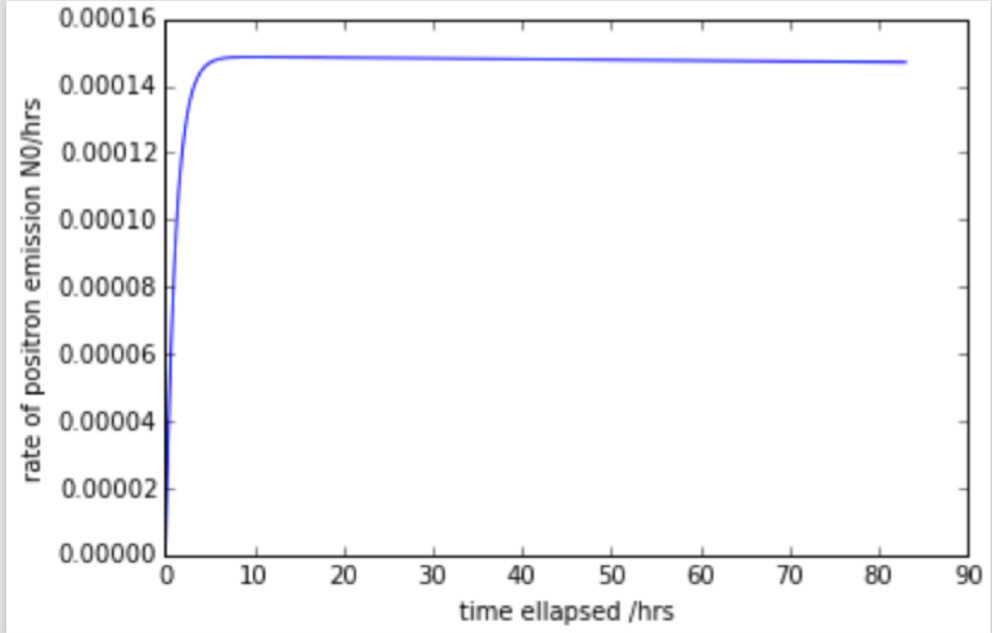
\includegraphics{Figures/C2F1}
\decoRule
\caption[C2F1]{The activity of the 68Ge/68Ga fuel as function of time. The units of y axis is the number of initial 68Ge atoms.}
\label{fig:C2F1}
\end{figure}

The ten hours that the sample takes to reach its full activity allows a reasonable time to transfer the sample from the point of production to the point of use. Transportation is required, since the production of 68Ge is a nuclear reaction and particle accelerators and nuclear sources are needed for its production. The activity drops to 90\% of its maximum roughly a month after it has reached it. Based on cost efficiency and other circumstances, such as safety, the slow rate of this decay in activity allows to choose a convenient period of time of the order of a month over which the sample has to be replaced by a new one in order to keep the activity high enough so stimulated emission is still possible (see below).

There are other, more complex ways of creating polarised positrons. These methods are costly and do not result in a significant raise in polarisation. They use circularly polarised $\gamma$ ray radiation for electron-positron pair creation. Two of these methods are the $\gamma$ ray radiation from helical ondulators and the use of Compton scattering. Appendix A contains an estimate on how much radioactive source is needed to be able to create a burst of 1kJ $\gamma$-ray laser. 

\section{Fuel Production}

There are many ways for producing 68Ge some of them are listed below:

\begin{equation}
\label{e4}
Ga^{nat} + \rho = Ge_{68} + xn
\end{equation}

\begin{equation}
\label{e5}
Ge^{nat} + \rho = Ge_{68} + p + xn
\end{equation}

\begin{equation}
\label{e6}
Zn^{nat} + \alpha = Ge_{68} + xn
\end{equation}

For 68Ge production simply the elementary form of each source is used disregarding the actual isotope content, hence the number of neutrons emitted during the reaction depends on the actual isotope that is struck by the incoming particle ($\rho$ or $\alpha$).
The actual reactions summarised in Fig. 2.1 and Fig. 2.2 [2]:

\begin{figure}[h]
\centering
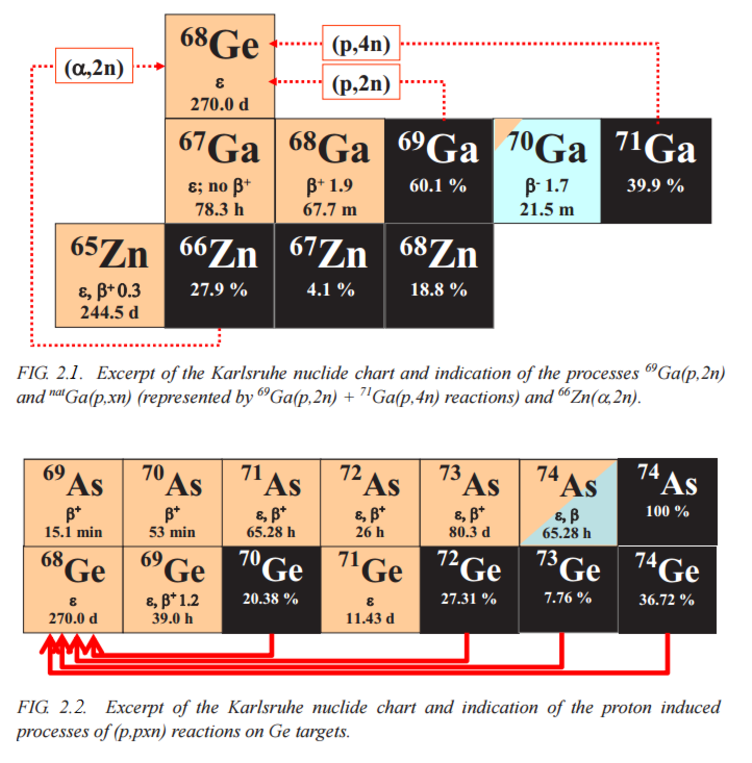
\includegraphics{Figures/C2F2}
\decoRule
\caption[C2F2]{Summarised Reactions}
\label{fig:C2F2}
\end{figure}

\begin{figure}[h]
\centering
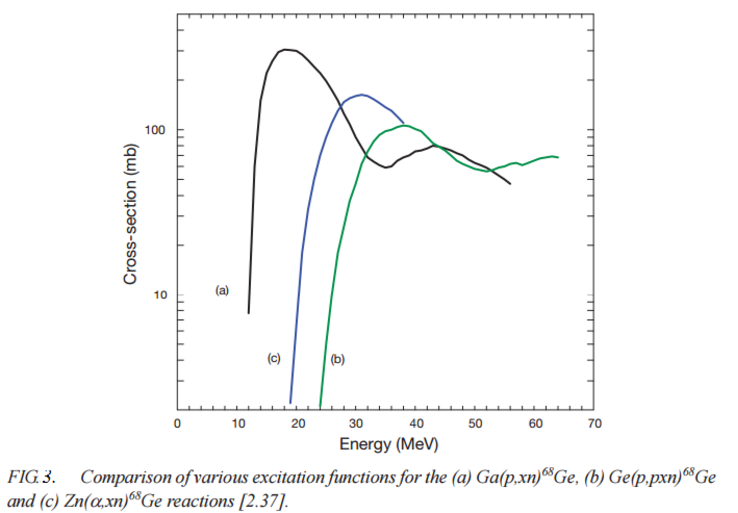
\includegraphics{Figures/C2F3}
\decoRule
\caption[C2F3]{Cross sections of each production paths against the energy of the projected incoming particle [2]}
\label{fig:C2F3}
\end{figure}

As the curves show, the best way to acquire is to use a Gallium source bombarded with protons of approximately 18MeV energy. This range of energy is easily achievable in many accelerators. For the Gallium reaction, the first maximum corresponds for a maximum in the partial cross section of the 69Ga(p,2n)68Ge reaction and the second local maximum corresponds to a peak in the partial cross section of the 71Ga(p,4n)68Ge. 

\section{Accumulation of Positrons}

The accumulation of a large number of positrons that are ready to be released in ultrashort pulses is essential in the creation of a $\gamma$-ray laser. Since the overall efficiency of the whole process is very low, i.e. most of the positrons radiated by the source will not participate in the stimulated emission, the more positrons available at the time of usage of the laser, the more likely that stimulated annihilation is achievable and also the more energy the output laser pulse will have. Most accumulation instruments comprise of an ultrapure neon moderator, a trap and an accumulator. The purpose of the neon moderator is to slow down the positrons to a few eV once it has left the source and radially compressed via the rotating wall technique. These slow positrons are then transported to a trap where they are radially confined. However, in order to prevent positrons returning to the moderator when transferred to the trap the moderator potential must be gradually increased at a steady rate.

\section{The Penning-Malmberg Trap}

One way to store positrons for a longer period of time is the use of the so called Penning-Malmberg trap (PM trap) [3]. There are many advantages of employing a PM trap, most importantly it is the long confinement times that allow the accumulation of large amounts of positron particles. Other advantages include: the potential for brightness enhancement by compressing the positron plasma and the ability to generate short positron pulses.
The main features of the PM trap is a strong axial magnetic field that confines the particles radially and a quadrupole field for axial confinement. An improved version of it is the multi-cell trap (MCT).Positrons can be stored for very long times in a plasma state with this device and also can be cooled and released in tailored bursts. The main challenge to overcome is the increasing space charge density upon accumulation that degrades confinement. 
To successfully trap the positrons an energy loss mechanism is required, the most common technique is the use of a buffer gas, which exploits inelastic scattering collisions between the particles. A lower electrostatic potential and gas pressure is obtained through the use of electrodes of increasing radii. The positrons when first passing through the trap are subject to a high gas pressure so that there are a greater number of collisions between the positrons. As the positrons progress through the higher stages they continue to collide with one another and the pressure of the buffer-gas is progressively reduced. This causes the temperature of the positrons to reduce down to room temperature in approximately 0.1 s. The most effective gas for this purpose is Nitrogen. At most 30\% of incoming positrons are trapped in the accumulator. Utilising this three stage buffer-gas trap enables the accumulation of several hundred million positrons with lifetimes of several minutes. 4x109 positrons have been confined at 1.2 K where the gas pressure is estimated to be less than or equal to 8x10-17 mbar [4].
Although there are alternative methods to using a buffer-gas, however, they are far less efficient. Such techniques are dependent upon the positron sources utilised, for example, to make use of the pulsed nature of a linac-based positron source the potential on one of the end caps is reduced allowing the positron pulse to enter the trap and then increasing the potential thus preventing the pulse from escaping. However, for our purposes the use of a buffer-gas is the most ideal. However, the one drawback from the use of a buffer-gas is that the gas molecules allow annihilation to occur thus reducing the storage time.
The aim here is to accumulate a large number of positron particles which are then delivered in pulses at a later time. Consequently, the critical issue of positron loss as a result of transport and annihilation must be considered. During a collision the wavefunctions of the positron and electron overlap causing them to annihilate. However, if a vacuum of good quality is used this is not a significant issue. Therefore, an ultra-high vacuum (UHV) environment is required to prevent annihilation. Alternatively we can reduce the loss of positrons by removing any grease, oil or other small quantities of large molecules from the system as otherwise positrons can attach themselves to these molecules, thus resulting in much higher rates of annihilation. Additionally, positron loss as a result of transportation is due to a torque exerted on the plasma due to the presence of any external force; the effect of this exerted torque is that it causes the plasma to expand radially. The viscous drag experienced by the plasma as a result of not only the collisions with the neutrally charged background gas but also the asymmetries of the trap caused by machining imperfections are examples of sources of such a torque.
In the multi-cell configuration, the plasma is divided into m parts, hence for a given confining potential, m times more particles can be stored. The positrons coming from the source are first compressed with the rotating wall technique[5]. The typical strength of magnetic fields used is approximately 5 T. The graphical design for the MCT is shown on Fig. 4.[6]

\begin{figure}[h]
\centering
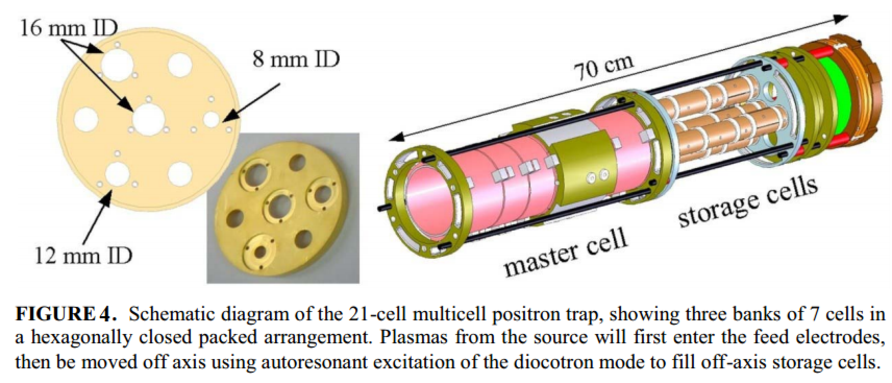
\includegraphics{Figures/C2F4}
\decoRule
\caption[C2F4]{Diagram of Multicell Positron Trap}
\label{fig:C2F4}
\end{figure}

This technique has been implemented to confine 109 particles for a time duration longer than a day [7]. The positrons are ejected from the trap in pulses. If parabolic potential is rapidly applied on an ensemble of positrons, they arrive at the target at roughly the same time and positron pulses with width of approximately 15-20ns can be created that contains over 106 particles. In order to lower the pulse width, a buncher is also introduced between the accumulator and the target. After introducing the buncher, the pulses are improved to have a width of approximately 1ns with a number of 70x106 positrons. The created positron plasmas have an areal density of typically 109 cm-2, which is still low for most of the Positronium interaction wished to be observed later. In order to produce the exotic Positronium atoms, subnanosecond pulses of positrons with a minimum density of 1x10'10 cm-2 [8] are required. For this reason the sample is further compressed by a pulsed magnetic field. The resulting density is in the range of (2-4) x 10'10 cm'-2.
The maximum number of positrons that can be stored in the MCT increases with the confining potential and the tube length of the cells. Fig. 5. shows the results of the experiment done by Danielson et al. on storing positrons.

\begin{figure}[h]
\centering
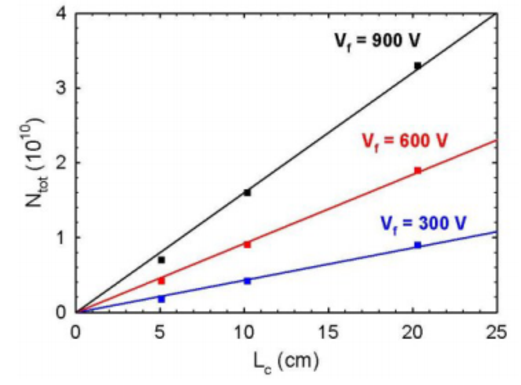
\includegraphics{Figures/C2F5}
\decoRule
\caption[C2F5]{The number of stored positrons as a function of the length of tubes used in the multicell conifguration for three different trapping voltages.}
\label{fig:C2F5}
\end{figure}

If it is assumed that 1 in every 1000 accumulated positrons will participate in the stimulated emission, the number of positrons need to be stored is in the order of 10'19 for achieving a pulse of gamma ray laser with an energy of 1 kJ. If the linear relationship between the stored positrons and cell length is assumed to be held for all cell length, for a trapping voltage of 900V a tube of length 62500km is required. Even if 1000 tubes are used, every one of them has to be 62.5km long that is equivalent to a circular tube with radius of 10km. Just for comparison, this is more than twice as long as the LHC at CERN. 
`	The length of the cells could be lowered significantly if higher trapping voltages were available, however raising the voltage can lead to a few complications. For example, higher voltages will result in heating that lowers the stability of the positron plasma due to the formation of Ps with the background neutral gas. 


\section{Decoupled Surko-Trap}

The areal density requirements for the positron pulses mentioned above are not only met but exceeded via the use of a decoupled Surko-trap, which is able to emit a beam of intense positrons of areal densities exceeding 3 x 10'10 cm-2   [8] in subnanosecond pulses. The Surko-type and the Penning-Malmberg trap share a lot of common features, for clarity purposes these are pointed out once more in the description for the Surko-trap below. Advantages of employing this variation of a Surko trap include the longer lifetimes of positrons and the cost reduction due to removing the need for large and expensive magnets and vacuum chambers.
From Fig. 6. [8] it can be seen that the decoupled Surko-trap of an approximate length of 5.5m consists of a positron source, a trap, an accumulator, a target chamber and a buncher. Positrons once leaving the source are subject to an ultrapure neon moderator, the purpose of this is to slow the positrons down to a few eV. However, the exposure of the moderator to the nitrogen buffer gas results in the beam intensity to be greatly reduced to approximately 4 x 10'6 e'+ s'(-1)  [8]. An axial magnetic field is then used to radially confine the positrons, and the presence of the electrostatic potential well confines the particles along the direction of the magnetic field.

\begin{figure}[h]
\centering
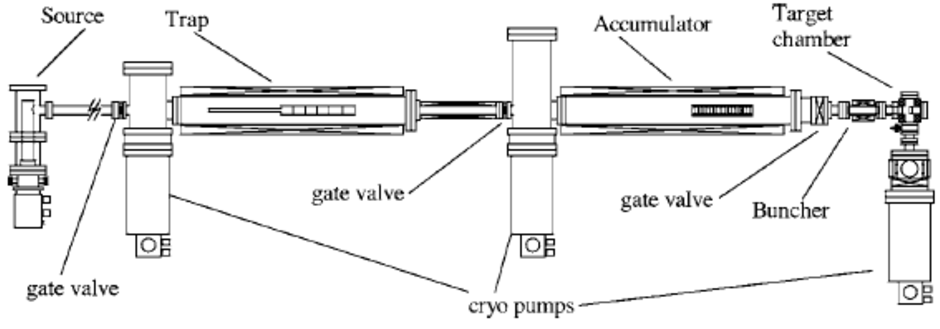
\includegraphics{Figures/C2F6}
\decoRule
\caption[C2F6]{Schematic diagram of the composition of all the components of the decoupled Surko-trap.}
\label{fig:C2F6}
\end{figure}

The positrons then enter a two-stage Surko-type trap infused with a buffer gas, as can be seen in Fig. 7. Stage 1 consists of a narrow electrode with an inside diameter of 8mm and stages 2a and 2b contains a segmented electrode with inside diameter 2.54cm, which allows the radial compression of positrons in stage 2b via a ‘rotating wall’ electric field. The positron cloud can be compressed to a final diameter of approximately 1.3mm full width at half maximum, where the rf is 5MHz, when a cooling gas (SF6 or CF4) [9]of a pressure of 20\% of that of the Nitrogen buffer gas is introduced. There is no significant loss in the lifetime of the positrons as a result of introducing a cooling gas [8].  
Stage 1 contains the Nitrogen buffer gas with an approximate pressure of 1x10'-3 Torr; the pressure of the gas is progressively reduced in stages 2a and 2b to an order of magnitude less than in stage 1, noting that there is very little difference in pressure across 2a and 2b. The lifetime of positrons are approximately 2s, and as a result of the short lifetime, the trap operates at 4Hz to maximise the number of particles passing through the trap. The efficiency of trapping using this particular method is approximately 20\% [8].

\begin{figure}[h]
\centering
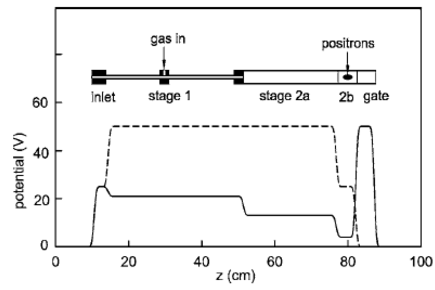
\includegraphics{Figures/C2F7}
\decoRule
\caption[C2F7]{Electrode structure of the buffer gas trap. The solid and dashed lines represent the potentials required for the trapping and releasing of positrons.}
\label{fig:C2F7}
\end{figure}

The positrons are then transferred to the accumulator and are trapped within a harmonic potential well. The positron loss is very low when the next pulse of positrons are transferred into the accumulator. As a result of cross-field transport, positrons have a typical lifetime of approximately 100s within the accumulator, however, this mechanism of positron loss has been eliminated via the ‘rotating wall’ technique.
The rotating wall in addition to counteracting the outward transport of the plasma, compresses the plasma. However, the plasma heats up as it is compressed, therefore a cooling mechanism, in the form of a cooling gas (SF6 or CF4) is needed at a pressure where there is no significant increase in the positron annihilation rate. The frequency of the rotating wall is approximately 4MHz and for a few seconds is then raised to 8MHz, thus allowing a containment of up to 95x10'6 positrons.
Using the techniques described the plasma areal densities achieved at the target are up to 2x10'-9 cm -2, however, the areal density can be further increased to (2-4) x 10'10 cm'-2 with the use of a pulsed magnetic field of approximately 1T which is applied at the target.
The plasma is transported from the accumulator using a parabolic potential which is able to eject the positrons at the same time, thus producing pulses of positrons which are restricted to a width of 15-20ns containing more than 1x10'6 positrons. Subnanosecond pulses are achieved with the application of a buncher, the structure of which can be seen in Fig. 8.[8] The buncher is positioned just before the positrons reach the target and is able to compress a maximum of 70x10'6 positrons into approximately a 1ns pulse [8].

\begin{figure}[h]
\centering
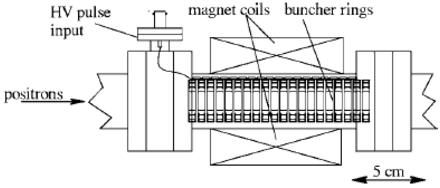
\includegraphics{Figures/C2F8}
\decoRule
\caption[C2F8]{Schematic diagram showing the structure of the buncher.}
\label{fig:C2F8}
\end{figure}

The use of a multiring accelerator enables the acceleration of the beam to approximately5kV, whilst eliminating additional positron losses as well as the associated gamma ray bursts.
To reiterate, the aim here is to accumulate a large number of positron particles which are then delivered in pulses at a later time. Consequently, the critical issue of positron loss as a result of transport and annihilation must be considered. We can take measures to reduce the loss of positrons by removing any grease, oil or other small quantities of large molecules from the system as otherwise positrons can attach themselves to these molecules, thus resulting in much higher rates of annihilation. Additionally, positron loss as a result of transportation is due to a torque exerted on the plasma in the presence of any external force; the effect of this exerted torque is that it causes the plasma to expand radially. The viscous drag experienced by the plasma as a result of not only the collisions with the neutrally charged background gas but also the asymmetries of the trap caused by machining imperfections are examples of sources of such a torque. [10]
The decoupled Surko-trap described is able to create 1ns pulses of approximately 60x10'6 low energy positrons, with areal densities of 3x10'10 cm-2. [8] However, in order to fulfil the final objective of creating a gamma-ray laser we require a mechanism of trapping a relatively greater magnitude of positrons than discussed above. Methods of rescaling the Surko trap can be considered to allow a larger quantity of positrons to be trapped. The rescaling has proved to be a limitation of the decoupled Surko trap; if it were to be scaled longitudinally it would produce plasmas that were long and thin and ultimately unstable. The idea of the multi cell configuration applied on the decoupled Surko-type trap could significantly raise the numbers achieved in positron accumulation.


\section{Beam Control}
The next objective after the accumulator is the tailoring of a positron beam that will provide suitable initial conditions within the silicon target to enable stimulated annihilation of a BEC sometime after impact. In particular the beam will need to reach a certain areal density, be of a sufficiently low temporal width, contain a large enough positron population and be sufficiently polarised. The polarisation of the beam will have already been set before beam extraction as will the total positron population, but the amount of positrons lost between the accumulator and the target will depend on the techniques used. Developments have been made on this subject by the group of D.B. Cassidy, the main features of the technique are described in [8].

The first of interest is the properties of the beam just after leaving the trap, and how these properties can be controlled. They are set by the techniques used to extract the stored positrons in the accumulator. The most effective way to get an intense pulse of positrons is to quickly switch the potential of the electric field within the accumulator from the harmonic confining potential to a parabolic shape in order to achieve longitudinal compression. This will force all the positrons forward in one very short pulse. This must be done in the smallest possible time period as to create a pulse that is temporally narrow as possible. The pulse in its original form after extraction can have a temporal width of around 15–20 ns [8], as has been achieved experimentally. To further compress this width, the beam will be first guided through the buncher apparatus where a pulsed voltage is applied in such a way as to create a harmonic like potential extremely rapidly. This forces the beam to further compress to subnanosecond scales of around 1ns [8]. The rise time of the pulse is very small compared to the pre buncher pulse width of the beam.

\section{Formation of Positronium Atoms and Molecules}

If an intense positron beam is incident of porous silica, Positronium molecule formation can be observed. Silica is used because of its low cost and because it is an insulator. Metals and semiconductors cannot be used due to the high number of free electrons their screening effect prohibits Ps formation. [Ps formation] Positrons interact with the electrons in the bulk of the material and form Positronium (Ps) atoms. Up to 40\% of incoming positrons can be transformed to Ps [11]. These atoms have a lifetime of <1ns within the material. However if it is made porous, the atoms can diffuse into the voids of the material, significantly raising their lifetimes.

The vacuum lifetime of Ps depends on its spin state. If it’s a singlet (called para-positronium, pPs) the lifetime is very short (125ps), hence atoms created in the singlet state decay technically immediately after formation. The triplet state (known as ortho-positronium, oPs) has a lifetime of 142ns that allows enough time for Ps-Ps interaction.  The overall probability of two atoms interacting is about 10\% [The production of molecular Ps]. These interaction can result in one the two outcomes:

\begin{equation}
\label{e7}
oPs + oPs = pPs +pPs
\end{equation}

\begin{equation}
\label{e8}
X+oPs+oPs=X+Ps2
\end{equation}

The former is called spin exchange quenching (SEQ) and the second is the molecular positronium formation.
Eventually all the positrons of the incident beam annihilate with the electrons of the material. There is a pulse of $\gamma$ rays immediately after the sample is irradiated by the positron beam coming from direct annihilation and the fast decay of pPs molecules.	After Ps-Ps interaction, annihilation takes place immediately since these mechanisms essentially turn long-lived triplet states into either pPs (SEQ) or molecular positronium (Ps2) that also annihilates technically immediately. Raising the incoming positron beam intensity hence lowers the lifetime of Ps atoms.

At room temperature, the molecule formation is approximately ten times more likely than SEQ that is hence a secondary process, however at higher temperature molecule formation is suppressed and SEQ becomes more significant. Also, as a study shows [12], the ratio of the different types of quenching depends on the geometrical structure of the target silica bulk. If the voids within the target material is randomly distributed molecule formation is enhanced, while if they are aligned in one particular dimension, SEQ is more likely. As temperature is increased in the first type of geometry, quenching is suppressed. This can be explained by the surface state of Ps. As temperature is increased, Ps atoms desorb from the surface and there is a lack of third body that is needed for molecule formation and lack of phonons needed for quenching in order to conserve energy. For the first geometry the discrete levels of the surface states cannot accommodate for the hyperfine structure (no SEQ) and if the temperature is high enough (no surface Ps, hence no Ps2 formation) there is no significant quenching. In the second geometry, there are no surface states due to the continuous levels in energy and thus quenching is temperature independent and can be considered entirely due to SEQ [13].

In order to create a Bose-Einstein Condensate (BEC) all sorts of quenching should be eliminated. For this purpose the size of the voids should be small enough so SEQ is suppressed and the temperature of the walls should be relatively high (room temperature or higher) so Ps atoms desorb from the surfaces and molecule formation is avoided. In order to achieve BEC a high density of particles is needed and hence the created Ps atoms should be collected somewhere within the material. Increased quenching effects due to the increased density should also be taken into account.

